\documentclass[twocolumn]{article}

\usepackage{imr}
\usepackage{graphicx}
\usepackage{amsfonts}
\usepackage{bbm}       % for \mathbbm{1}
\usepackage{amsmath}
\usepackage{mathrsfs}  % for \mathscr
\usepackage{tikz}
\usetikzlibrary{decorations.markings}

\def\thepage {}
\bibliographystyle{imr}

\begin{document}

\title{An ergonomic approach to topological transformations of unstructured meshes}
\author{Daniel Shapero$^1$}
\date{
    $^1$University of Washington, Seattle, WA, USA, shapero@uw.edu
}

\abstract{In this paper, we will describe a new approach to performing local transformations to the topology of an unstructured mesh.
Our approach borrows some ideas from algebraic topology and makes for much easier verification of the underlying computational kernels.}

\keywords{mesh generation, computational geometry, topology}

\maketitle
\thispagestyle{empty}
\pagestyle{empty}


% --------------------
\section{Introduction}

All algorithms for generating unstructured meshes are based on using a sequence of local transformations of the mesh topology.
The simplest of these transformations is a 2-2 edge flip, which is the basis of one common algorithm for computing the Delaunay triangulation of a planar point set \cite{lawson1972transforming}.
In 3D, these generalize to 3-2 and 2-3 tetrahedral flips, and in arbitrary dimensions these are called bistellar flips or Pachner moves \cite{pachner1991pl}.
An alternative algorithm for Delaunay triangulation instead uses deletion and retriangulation of star-shaped polytopes \cite{bowyer1981computing, watson1981computing}.

Implementing these topological transformations can be difficult and error-prone.
In this paper, we will describe a new method for implementing local topological transformations using ideas from algebraic topology.
We refer to \cite{hatcher2002algebraic} for all formal definitions.
Our method is based on representing the \emph{boundary operators} of a \emph{chain complex}.
These boundary operators are really just matrices with integer coefficients.
We can then describe transformations using linear algebra.


% -----------------------
\section{Chain complexes}

The end goal of mesh generation is to construct a simplicial complex.
A natural way to represent a simplicial complex might be, say, a doubly-connected edge list; a 2D integer array, storing the ordered vertices of each top-dimensional simplex; or any number of other related data structures.
We will instead take the unconventional step of using more general \emph{cell complexes}.
We'll motivate the idea by first considering the simplicial case.

Recall that, given an ordered $k$-simplex $[v_0, \ldots, v_k]$, the \emph{boundary} of this simplex is a formal integer linear combination of $k - 1$-simplexes:
\begin{equation}
    \partial[v_0, \ldots, v_k] = \sum_i(-1)^i[v_0, \ldots, \hat v_i, \ldots, v_k]
    \label{eq:simplicial-boundary}
\end{equation}
where $[v_0, \ldots, \hat v_i, \ldots, v_k]$ is the simplex obtained by removing the vertex at index $i$.
Now define a $\mathbb{Z}$-module $\mathscr{C}_k$ consisting of all formal integer linear combinations of simplexes of degree $k$.
Elements of this module are called \emph{chains} or $k$-chains when we need to refer to the dimension explicitly.
Extending definition \eqref{eq:simplicial-boundary} by $\mathbb{Z}$-linearity, we can prove that $\partial_k : \mathscr{C}_k \to \mathscr{C}_{k - 1}$ is a module homomorphism and
\begin{equation}
    \partial_k\cdot\partial_{k + 1} = 0.
    \label{eq:ddzero}
\end{equation}
The natural data structure to represent a boundary operator is a sparse matrix with integer coefficients.

\textbf{A chain complex is any sequence of $\mathbb{Z}$-modules $\mathscr{C}_k$ together with a set of linear operators $\partial_k$ satisfying equation \eqref{eq:ddzero}.}
A simplicial complexes naturally gives rise to a chain complex, but so can other types of geometries.
For example, we can define boundary operators on cubical or polygonal complexes that satisfy equation \eqref{eq:ddzero}.
The $k$-th boundary operator for a simplicial complex has a kind of regularity in that every column has $k + 1$ non-zero entries, but this regularity is not essential in general.
See figure \ref{fig:two-triangle-chain-complex} for an illustration of a simple topology together with the corresponding boundary operators.

% TODO: Add labels to the figure and the boundary matrices, see
% https://tex.stackexchange.com/a/59732
\begin{figure}[h]
    \begin{minipage}{0.48\linewidth}
        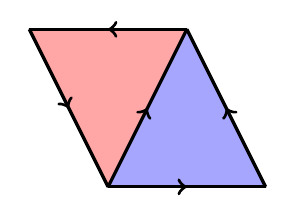
\begin{tikzpicture}
            \draw[fill=blue!35] (1, 0) -- (3, 0) -- (2, 2) -- cycle;
            \draw[fill=red!35] (1, 0) -- (2, 2) -- (0, 2) -- cycle;
            \begin{scope}[
                very thick,
                decoration={markings, mark=at position 0.5 with {\arrow{>}}}
            ]
                \draw[postaction={decorate}] (1, 0) -- (3, 0);
                \draw[postaction={decorate}] (3, 0) -- (2, 2);
                \draw[postaction={decorate}] (2, 2) -- (0, 2);
                \draw[postaction={decorate}] (0, 2) -- (1, 0);
                \draw[postaction={decorate}] (1, 0) -- (2, 2);
            \end{scope}
        \end{tikzpicture}
    \end{minipage}
    \hfill
    \begin{minipage}{0.48\linewidth}
        {\small
            \begin{equation*}
                \partial_1 = \left[\begin{matrix}
                    - &   & + & - &   \\
                    + & - &   &   & + \\
                      & + & - &   &   \\
                      &   &   & + & -
                \end{matrix}\right]
            \end{equation*}
            \begin{equation*}
                \partial_2 = \left[\begin{matrix}
                    + & - \\
                    + &   \\
                    + &   \\
                      & + \\
                      & +
                \end{matrix}\right]
            \end{equation*}
        }
    \end{minipage}
    \caption{Pair of adjacent triangles (left) and their boundary matrices (right).}
    \label{fig:two-triangle-chain-complex}
\end{figure}

We'll introduce one final conceit that makes later constructions much more elegant.
The definition above assumes that the chain complex stops at $\mathscr{C}_0$ -- formal linear combinations of vertices.
Instead, we will add a \emph{bottom} module $\mathscr{C}_{-1}$ consisting of a single cell $\bot$ of dimension -1.
We then define the boundary of every vertex $v_i$ to be $+\bot$.
If we write $\mathbbm{1}$ for the column vector of all 1s, then $\partial_0 = \mathbbm{1}^*$, i.e. the row vector of all 1s.
The addition of this bottom cell is especially convenient because the condition $\partial_0\partial_1 = 0$ implies that the boundary of every edge $e$ has a negative and a positive vertex: $\partial e = v_i - v_j$ for some $i$, $j$.
We cannot have, for example, $\partial e = v_i + v_j$, which would be undesirable.

Given the boundary matrices $D_0, \ldots, D_k$ of a single simplex, one can recover the equivalent ordering $[v_0, \ldots, v_k]$ of its vertices.
By applying this recovery procedure for every top-dimensional cell, one can translate back from the chain complex representation, which is best suited to transforming the topology, to the simplicial representation, which is better for finite element analysis or graphical rendering.


% -----------------------
\section{Transformations}

The goal of using chain complexes and boundary operators is to represent all local transformations through purely linear algebraic means.
Phrasing the problem in this way makes verifying correctness easy.

\subsection{Merging}

First, observe that if $A$, $B$ are integer matrices such that the image of $A\cdot B$ is in the image of $\partial_{k + 1}$, then the matrices
\begin{equation}
    \partial_k' = \partial_k\cdot A, \quad \partial_{k + 1}' = B\cdot\partial_{k + 1}
\end{equation}
still satisfy $\partial_k'\cdot\partial_{k + 1}' = 0$.
A particular case is $A\cdot B = I$, which includes for example permutations of the cells.
The more general case regarding the image of $A\cdot B$ is needed for some irreversible transformations.

A \emph{merge} of adjacent $k$-cells replaces them with a single cell.
Merging is a column operation, i.e. right multiplication, on the matrix $\partial_k$.
Adjacent top-dimensional cells can be merged freely and the new boundary operator is
\begin{equation}
    \partial_n' = \partial_n\cdot\mathbbm{1}.
\end{equation}
Strictly speaking, we should also impose a condition that the union of the cells to be merged is simply-connected.
One might imagine triangulating an annulus and then merging all the cells together; the union is no longer simply-connected, which violates one of the conditions to be a cell complex (see \cite{hatcher2002algebraic}).
In realistic problems, for example in implementing the Bowyer-Watson algorithm, one can often prove that a set of cells to be merged form a star-shaped polygon.

For cells that are not top-dimensional, we might need to instead flip some signs, in which case the transformation is
\begin{align}
    \partial_k' & = \partial_k\cdot\text{diag}(s_0, \ldots, s_m)\cdot\mathbbm{1}, \\
    \partial_{k + 1}' & = \left[\begin{matrix} 0 \ldots 1 \ldots 0\end{matrix}\right]\partial_{k + 1}.
\end{align}
where $s_i$ are all $\pm 1$.
The transformation to the rows of $\partial_{k + 1}$ collapses all incidence to any of the desired $k$-cells into incidence to the merged $k$-cell.

\subsection{Splitting}

A \emph{split} divides up the union of several polytopes along a point.
The key correctness criteria for this operation are that (1) every newly-created polytope contains the splitting point and (2) the boundary of the sum of all polytopes does not change.
We'll first describe the 2D case and then proceed to arbitrary dimensions.

Suppose that a collection of adjacent polygons has the boundary operators $\partial_1$ and $\partial_2$.
We first have to draw edges between the new vertex and all the vertices of the polygon.
The orientation of these new edges is arbitrary, so we can assume that every edge goes from the splitting vertex $v$ to the polygon vertices.
Another way of stating this is that every new edge $e$ is negatively-incident to $v$ and positively-incident to some polygon vertex.
In terms of matrices, the new 1-boundary operator is
\begin{equation}
    \partial_1' = \left[\begin{matrix}\partial_1 & I \\ 0 & -\mathbbm{1}^*\end{matrix}\right]
    \label{eq:split-1-2d}
\end{equation}
where $I$ is the identity matrix.
The key step here is defining the 2-boundary matrix:
\begin{equation}
    \partial_2' = \left[\begin{matrix}\text{diag}(\partial_2\cdot\mathbbm{1}) \\ -\partial_1\cdot\text{diag}(\partial_2\cdot\mathbbm{1})\end{matrix}\right]
\end{equation}
A rudimentary calculation shows that $\partial_1'\partial_2' = 0$.
Since $\text{diag}(z)\cdot\mathbbm{1} = z$ for any vector $z$, we also find that
\begin{equation}
    \partial_2'\mathbbm{1} = \left[\begin{matrix}\partial_2\mathbbm{1} \\ 0\end{matrix}\right]
\end{equation}
or in other words the new polygon has the same boundary as the old.
Figure \ref{fig:split-transformation} illustrates the split transformation on a single quadrilateral and shows the boundary matrices before and after.

\begin{figure}[h]
    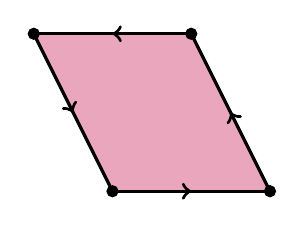
\begin{tikzpicture}
        \coordinate (p0) at (1.5, 1){};
        \coordinate (p1) at (1, 0){};
        \coordinate (p2) at (3, 0){};
        \coordinate (p3) at (2, 2){};
        \coordinate (p4) at (0, 2){};

        \draw[fill=purple!35] (p1) -- (p2) -- (p3) -- (p4) -- cycle;
        \begin{scope}[
            very thick,
            decoration={markings, mark=at position 0.5 with {\arrow{>}}}
        ]
            \draw[postaction={decorate}] (p1) -- (p2);
            \draw[postaction={decorate}] (p2) -- (p3);
            \draw[postaction={decorate}] (p3) -- (p4);
            \draw[postaction={decorate}] (p4) -- (p1);
        \end{scope}

        \foreach \p in {p1, p2, p3, p4} {
            \filldraw (\p) circle (2pt);
        }
    \end{tikzpicture}
    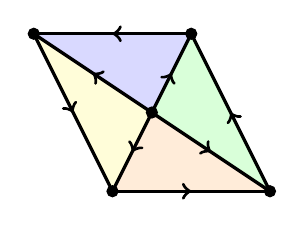
\begin{tikzpicture}
        \coordinate (p0) at (1.5, 1){};
        \coordinate (p1) at (1, 0){};
        \coordinate (p2) at (3, 0){};
        \coordinate (p3) at (2, 2){};
        \coordinate (p4) at (0, 2){};

        \draw[fill=orange!15] (p1) -- (p2) -- (p0) -- cycle;
        \draw[fill=green!15] (p2) -- (p3) -- (p0) -- cycle;
        \draw[fill=blue!15] (p3) -- (p4) -- (p0) -- cycle;
        \draw[fill=yellow!15] (p4) -- (p1) -- (p0) -- cycle;
        \begin{scope}[
            very thick,
            decoration={markings, mark=at position 0.5 with {\arrow{>}}}
        ]
            \draw[postaction={decorate}] (p1) -- (p2);
            \draw[postaction={decorate}] (p2) -- (p3);
            \draw[postaction={decorate}] (p3) -- (p4);
            \draw[postaction={decorate}] (p4) -- (p1);
            \draw[postaction={decorate}] (p0) -- (p2);
            \draw[postaction={decorate}] (p0) -- (p3);
            \draw[postaction={decorate}] (p0) -- (p4);
            \draw[postaction={decorate}] (p0) -- (p1);
        \end{scope}

        \foreach \p in {p0, p1, p2, p3, p4} {
            \filldraw (\p) circle (2pt);
        }
    \end{tikzpicture}

    {\small
        \begin{equation*}
            \partial_1 = \left[\begin{matrix}
                - &   &   & + \\
                + & - &   &   \\
                  & + & - &   \\
                  &   & + & -
            \end{matrix}\right],
            \quad
            \partial_2 = \left[\begin{matrix}
                + \\ + \\ + \\ +
            \end{matrix}\right]
        \end{equation*}

        \begin{equation*}
            \partial_1' = \left[\begin{array}{cccc|cccc}
                - &   &   & + & + &   &   &   \\
                + & - &   &   &   & + &   &   \\
                  & + & - &   &   &   & + &   \\
                  &   & + & - &   &   &   & + \\
                \hline
                  &   &   &   & - & - & - & -
            \end{array}\right]
        \end{equation*}
        \begin{equation*}
            \partial_2' = \left[\begin{array}{cccc}
                + &   &   &   \\
                  & + &   &   \\
                  &   & + &   \\
                  &   &   & + \\
                \hline
                + &   &   & - \\
                - & + &   &   \\
                  & - & + &   \\
                  &   & - & +
            \end{array}\right]
        \end{equation*}
    }

    \caption{Quadrilateral before and after splitting on a new vertex in the center (top) and boundary matrices before and after (bottom).}
    \label{fig:split-transformation}
\end{figure}

We can get an idea for how to extend this to $n$ dimensions by remembering that $\mathbbm{1}^* = \partial_0$ in equation \eqref{eq:split-1-2d}.
This suggests the transformation
\begin{align}
    \partial_k' & = \left[\begin{matrix}\partial_k & I \\ 0 & -\partial_{k - 1}\end{matrix}\right] \label{eq:split-k} \\
    \partial_n' & = \left[\begin{matrix}\text{diag}(\partial_n\cdot\mathbbm{1}) \\ -\partial_{n - 1}\text{diag}(\partial_n\cdot\mathbbm{1})\end{matrix}\right] \label{eq:split-n}
\end{align}
Again, a rudimentary calculation shows that the fundamental equation \eqref{eq:ddzero} still holds and that the new polytopes have the same boundary as the old.
To our knowledge, equations \eqref{eq:split-k} and \eqref{eq:split-n} have not appeared in the literature before.
All the primitive construction operations required to form these matrices are available in the NumPy linear algebra module \cite{harris2020array}.

\subsection{Splitting and merging}

The split transformation is all that is required to implement the Bowyer-Watson algorithm \cite{bowyer1981computing, watson1981computing} or to compute convex hulls \cite{berg1997computational}.
Other transformations can be defined by combining a sequence of splits and merges.
For example, a 2-2 flip in 2D can be defined by (1) splitting the quadrilateral along a temporary, virtual vertex, (2) merging two pairs of triangles, (3) merging two edges to form the diagonal, and finally (4) deleting the virtual vertex.
Similarly, 2-3 and 3-2 flips can be implemented by first going through an intermediate state consisting of 6 tetrahedra.

\begin{figure}[h]
    \tikzset{ec/.style={every coordinate/.try}}

    \begin{tikzpicture}[scale=0.4]
        \coordinate (p0) at (1.5, 1){};
        \coordinate (p1) at (1, 0){};
        \coordinate (p2) at (3, 0){};
        \coordinate (p3) at (2, 2){};
        \coordinate (p4) at (0, 2){};

        \begin{scope}[very thick]
            \draw (p1) -- (p2) -- (p4) -- cycle;
            \draw (p4) -- (p3) -- (p2) -- cycle;

            \foreach \p in {p1, p2, p3, p4} {
                \filldraw (\p) circle (3pt);
            }
        \end{scope}

        \begin{scope}[very thick, every coordinate/.style={shift={(3.5,0)}}]
            \draw ([ec]p1) -- ([ec]p2) -- ([ec]p3) -- ([ec]p4) -- cycle;

            \foreach \p in {p1, p2, p3, p4} {
                \filldraw ([ec]\p) circle (3pt);
            }
        \end{scope}

        \begin{scope}[very thick, every coordinate/.style={shift={(7,0)}}]
            \draw ([ec]p0) -- ([ec]p1) -- ([ec]p2) -- cycle;
            \draw ([ec]p0) -- ([ec]p2) -- ([ec]p3) -- cycle;
            \draw ([ec]p0) -- ([ec]p3) -- ([ec]p4) -- cycle;
            \draw ([ec]p0) -- ([ec]p4) -- ([ec]p1) -- cycle;

            \foreach \p in {p0, p1, p2, p3, p4} {
                \filldraw ([ec]\p) circle (3pt);
            }
        \end{scope}

        \begin{scope}[very thick, every coordinate/.style={shift={(10.5,0)}}]
            \draw ([ec]p1) -- ([ec]p2) -- ([ec]p3) -- cycle;
            \draw ([ec]p3) -- ([ec]p4) -- ([ec]p1) -- cycle;

            \foreach \p in {p0, p1, p2, p3, p4} {
                \filldraw ([ec]\p) circle (3pt);
            }
        \end{scope}

        \begin{scope}[very thick, every coordinate/.style={shift={(14,0)}}]
            \draw ([ec]p1) -- ([ec]p2) -- ([ec]p3) -- cycle;
            \draw ([ec]p3) -- ([ec]p4) -- ([ec]p1) -- cycle;

            \foreach \p in {p1, p2, p3, p4} {
                \filldraw ([ec]\p) circle (3pt);
            }
        \end{scope}
    \end{tikzpicture}
    \caption{A 2-2 flip, implemented as a sequence of merges and splits.}
\end{figure}

A few papers have argued for the utility of multi-cell transformations for 3D mesh improvement \cite{klingner2008aggressive}.
Multi-cell transformations are substantially more complex than 2-3 or 3-2 flips, but \cite{misztal2009tetrahedral} showed that these complex transformations are implementable as a sequence of 2-3 and 3-2 flips.
Using the boundary operator representation might make it possible to implement complex topological transforms with less effort and in fewer steps.


% ------------------
\section{Conclusion}

Many data structures have been created to represent unstructured meshes and each one is designed to be optimal for particular use cases.
Doubly-connected edge lists have historically been very popular for mesh generation because they make traversal of the topology particularly simple.
Array-based representations, on the other hand, have seen more use in finite element analysis.
This representation is the most memory efficient and memory access is the performance-limiting factor for this application.
Here we propose that the boundary operators between chain complexes are an ideal representation for the local topology if the goal is to perform topological transformations.
When the underlying objects of study can be represented as linear operators, we can apply linear algebraic reasoning and intuition to define transformations and easily verify that they preserve all of the important invariants.
The condition in equation \eqref{eq:ddzero} that the product of two boundary operators is zero is a very powerful invariant for ensuring the validity of the underlying topology.


\bibliography{chain-complexes.bib}

\end{document}
